\subsection{La contribution au réchauffement climatique}


Après leur extraction, les matières premières sont rassemblées, transportées, puis transformées en d'autres composés, qui seront eux-même possiblement traités ou consommés dans des processus divers et variés. Tout cela a malheureusement un coût parfois important pour l'environnement.


\subsubsection{Le transport lié aux matières premières et produits finis : }
Le transport est un élément important pour le modèle de l'\op. En effet, il s'agit d'avoir un apport régulier de biens pour la vente, sinon, produire en continu ne servirait pas. On distingue ainsi plusieurs phases d'acheminement des produits.

La première est le transport des matières premières depuis le lieu d'extraction jusqu'aux usines de transformation. Les principaux pays exportateurs sont situés en Amérique du Sud et en Afrique. En effet les pays du nord ont consommé la plupart des leurs (charbon, mines de métaux), ou certaines normes de sécurité de l'environnement ne leur permettent pas d'extraire pour peu cher, et il devient plus avantageux pour eux d'acheter à l'étranger, puis d'amener ces ressources aux lieux de production. La destination phare est l'Asie de l'est, "L'Atelier du Monde", où la plupart des produits sont manufacturés.

Ces produits sont ensuite envoyés essentiellement dans les pays du nord, Europe et Amérique du Nord. Ils seront stockés dans des entrepôts, puis de nouveau transportés vers les lieux d'achats (supermarchés, boutiques). 

Et finalement, les produits consommés et mis à la poubelle sont emmenés vers une décharge et parfois malheureusement ceux-ci finissent en décharge sauvage en Afrique, comme au Ghana (voir partie suivante). Ils restent ainsi sans traitement et polluent durant de nombreuses années.

On a ainsi des bateaux, trains, avions, camions qui se déplacent à travers le monde afin de délivrer leurs produits. Cela induit de fait une pollution liée le plus souvent au CO2 éjecté par les moteurs des différents moyens de transport. Selon le GESAMP, le transport maritime compterait pour 12\% de la pollution qui touche les océans, comme le montre la figure \ref{PollutionMaritime}.

\begin{figure}[h]
\centerline{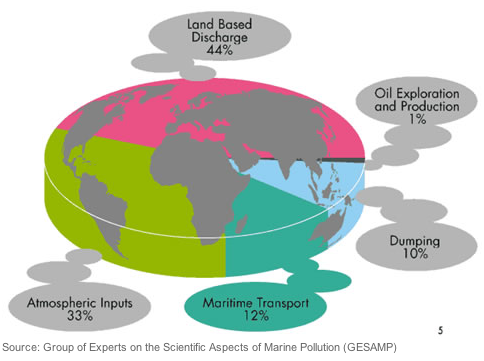
\includegraphics[scale=0.75]{Rsc/pollution_maritime.png}}
\caption{Graphique présentant la part de différents secteurs économiques ou environnementaux dans la pollution maritime}
\label{PollutionMaritime}%attention, à placer après le caption, sinon référencera la section
\end{figure}

L'obsolescence programmée, dans sa demande constante, oblige donc certaines entreprises à acheminer toujours plus de produits, et donc de matières premières, créant encore plus de pollution.

\bigbreak Après le transport, les ressources sont utilisées, brûlées ou transformées pour créer le produit fini. Nous allons voir à travers quelques exemples que cela est particulièrement coûteux au niveau écologique.


\subsubsection{L'utilisation des ressources à travers la production : }

Beaucoup de matériaux sont traités à l'aide de produits chimiques. En effet ceux-ci peuvent effectuer plusieurs actions, telles que : 
\begin{itemize}
  \item un collage : entre plusieurs matériaux de même nature ou non. 
  \item un nettoyage : pour enlever des impuretés, retirer des produits actifs
  \item une protection : contre le soleil, la pluie, les chocs, d'autres produits
\end{itemize}

On a ainsi un exemple d'utilisation indirecte de ressources naturelles dans la fabrication d'un produit. Ces produits chimiques étant bien entendu eux aussi élaborés à l'aide de matières premières. 

\medbreak Un deuxième exemple est l'aluminium, grand consommateur de produits et d’énergie dans sa conception.

Celui-ci se présente en premier lieu sous forme de minerai de bauxite. Extrait dans des mines d'Afrique, d'Amérique Latine et d'Australie principalement \cite{aluZonesExtraction}, puis transporté vers des usines. Là, différents procédés sont utilisés, le plus connu étant le Procédé Bayer dans lequel de la soude est principalement utilisée. On transforme ainsi quatre tonnes de bauxite en deux tonnes d'alumine. 

Puis celle-ci subit une dissolution dans une cuve. Un courant y est appliqué dans une réaction d'électrolyse afin de séparer l'aluminium et l'oxygène, composant l'alumine. Une seule tonne est ainsi produite à partir des deux tonnes d'alumine. Cette réaction est néfaste envers l'environnement pour deux raisons. La première est la rejet de CO2 dans l'atmosphère. Celui-ci provient de l'oxygène présent dans l'alumine et du carbone de l'anode de graphite. La principale est la deuxième raison : l'utilisation massive d’électricité lors de l'électrolyse. Selon l'Association de l'Aluminium du Canada \cite{consomUsinesAlu}, leurs usines nécessitent pas loin de 500 MégaWatts d’électricité pour fonctionner. Or une centrale telle que celle de Flamanville a une puissance de 2 600 MW. Cela signifie que chaque usine d'aluminium utilise un cinquième d'une installation nucléaire. Cela correspond à la consommation d'une ville comme Dunkerque.
Cet aluminium peut cependant encore être recyclé. Appelé alors secondaire, il ne représente que 20\% de la production dans le monde \cite{worldAluProdRecycl}. 

\bigbreak On a donc un épuisement des matières premières directement utilisées, mais également celles utilisées indirectement dans le transport (pétrole principalement) ou dans la conception des produits. Ceux-ci sont finalement jetés et finissent la plupart du temps dans une décharge où ils pourrissent sans aucun traitement.

